\input{style/settings}
\input{style/short_commands}
\pagestyle{fancy}
\fancyhf{}
\fancyhead[R]{página\;\thepage/\pageref{LastPage}}
\fancyhead[L]{Osvaldo Uriel Calderón Dorantes}
\fancyfoot[L]{Imagenología Biomédica}
\fancyfoot[R]{Facultad de Ciencias, UNAM 
\includegraphics[scale=0.13]{style/Sheikah.pdf}}
\fancypagestyle{plain}{
  \fancyfoot[C]{}
}
\makeatletter
\def\@seccntformat#1{%
  \expandafter\ifx\csname c@#1\endcsname\c@section\else
  \csname the#1\endcsname\quad
  \fi}
\makeatother
%%%%%%%%%%%%%%%%%%%%%%%%%%%%%%%%%%%%%%%%%%%%%%%%%%%%%%%
%%%%%%%%%%%%%%%%%%%%%%%%%%%%%%%%%%%%%%%%%%%%%%%%%%%%%%%%%%%
\begin{document}
\begin{flushleft}
Osvaldo Uriel Calderón Dorantes, \hfill Imagenología Biomédica\\
316005171 \hfill osvaldo13576@ciencias.unam  \\
Facultad de Ciencias\\
\underline{Universidad Nacional Autónoma de México}
\end{flushleft}

\begin{flushright}\vspace{-5mm}

\includegraphics[height=1.5cm]{style/logo.pdf}
\end{flushright}
 
\begin{center}\vspace{-1cm}
\textbf{ \large \customfont{Examen 1\\
Módulo RADIODIAGNÓSTICO}}\\
\today
\end{center}
%\medskip\hrule\medskip
%%%%%%%%%%%%%%%%%%%%%%%%%%%%%%%%%%%%%%%%%%%%%%%%
%{\small \textbf{Nota: A las unidades las pondré dentro de corchetes \ec{[\tx{unidad}]} para no confundir entre variables y realizar el análisis dimensional fácilmente.}}
\medskip\hrule\bigskip

\newlength{\strutheight}
\settoheight{\strutheight}{\strut}


\begin{enumerate}[1.]
\item Defina qué es el rendimiento fluorescente.

El rendimiento de fluorescencia \ec{\Phi} es un concepto de cuántico y se refiere a la eficiencia de la emisión de fotones a través de la fluorescencia, o bien,  la energía de una sustancia que ha perdido debido a la absorción de fotones y se define como se define como la relación entre el número de fotones emitidos y el número de fotones absorbidos dada en la ec. \ref{e:p1}, visto de otra manera, nos dice la probabilidad de que el estado excitado sea apagado debido a la fluorescencia.
\eq{e:p1}{\Phi=\dfrac{N(\tx{fotones emitidos})}{N(\tx{fotones absorbidos})}}


\item  Qué es el efecto fotoeléctrico. Haga un esquema y diga cuál es la importancia del mismo en las imágenes por rayos X.
\ftikz{1}{figuras/p2.tikz}{Esquema del efecto fotoeléctrico.}{fig:p2}
%vid1

Es un efecto que se produce entre los electrones de las capas internas del átomo (estrechamente unidos) y fotones de rayos X incidentes, este fotón es completamente absorbido por dicho electrón y se expulsa un fotoelectrón. La energía de este fotoelectrón es igual a la diferencia entre la energía del fotón incidente y la energía de enlace del electrón. En la figura \ref{fig:p2} tenemos el diagrama del efecto fotoeléctrico, el efecto se describe a continuación:
\begin{enumerate}[(a)]
  \item Incide un fotón de rayos X y es totalmente absorbido por algún electrón de la capa interna.
  \item Luego, éste es expulsado como un fotoelectrón, quedando una vacante.
  \item Esta vacante debe ser llenada por algún otro electrón, pero de la capa externa. Esto provoca una diferencia de energía, dando dos casos posibles:
  \item La energía se emite  como una radiación característica.
  \item O bien, se emite como electrón Auger, ya que la energía de los electrones de las capas externas es menor que la energía de transición del electrón del paso (c).
\end{enumerate}


¿Por qué es importante este efecto en las imágenes? Permite la obtención de imágenes de  tejidos tejidos blandos con fotones con energía por debajo de \ec{50 [keV]}. Además,  la absorción fotoeléctrica permite mostrar las diferencia, las cuales aumentan, entre la atenuación de los distintos tejidos en nuestro cuerpo, lo cual permite definir el contraste de la imagen.

\pagebreak

\item Describa el principio de funcionamiento de un tubo de rayos X y haga un esquema señalando sus partes. Además haga la descripción de la formación de una imagen con los 4 pasos, mencionados en clase.

\ftikz{1}{figuras/p3.tikz}{Esquema del tubo de rayos X.}{fig:p3}


En la figura \ref{fig:p3} muestra de los elementos necesarios para la generación de rayos X dentro de un tubo al vacío (esto para que no haya interacciones entre electrones y fotones con posible contaminación dentro del tubo): Se aplica una corriente la cual pasa por el filamento de tungsteno y éste es calentado, entonces, este calentamiento produce un aumento de energía que permite a los electrones que sean liberados del filamento a través por el efecto  termoiónico. Luego, estos electrones serán atraídos por el ánodo  y chocarán con el blanco de tungsteno con una energía dada por la diferencia de potencial aplicada a través de la fuente de alto voltaje, estos choques provocarán la radiación de frenado o el Bremsstrahlung y otras interacciones que dan lugar a los rayos X característicos.  Se emplea tungsteno ya que posse un alto punto de fusión  (\ec{3422^\circ C}) ya que se trata de un proceso ineficiente donde el \ec{99\%} de la energía se transforma en calor y  el \ec{1\%} se utiliza para la producción de rayos X.



Pasos para la formación de imágenes:
\begin{itemize}
  \item \textbf{Sujeto}: Es el porqué del uso de la imagenología, éste será el objeto de interés y físicamente se tratará como una distribución de los coeficientes lineales de atenuación en función del espacio y el tiempo.
  \item \textbf{Generador de portadores}: Nos dará la información que nos llevará a la formación de la imagen, los portadores pueden ser producidos fuera del sujeto (como por ejemplo, los tubos de rayos X) o dentro del sujeto (como por ejemplo, al administrar un radiofármaco con la emisión de fotones \ec{\gamma}.).
  \item \textbf{Detector}: Permitirá capturar la información que proviene de los portadores, debe ser capaz de dar un formación de posición y de número, para la información de energía será necesaria la capa hemirreductora.
  \item \textbf{Observador}: El observador, quien conoce el sistema anatómico del paciente, usará el sistema de visualización  e interpretará la imagen para determinar si hay alguna anomalía o lesión en el paciente.
\end{itemize}






\item Haga un esquema de la conversión interna.
%vid_1
\ftikz{1}{figuras/p4.tikz}{Diagrama de conversión interna.}{fig:p4}
%Durante la desintegración/decaimiento del núcleo en vez de expulsar el rayo gamma hacia el exterior del átomo, es "absorbido" por el átomo y origina una “colisión” con un electrón de las capas internas (capa K), es decir le transfiere energía al electrón y este sale expulsado.

\pagebreak

De acuerdo a la figura \ref{fig:p4}, 
cuando un núcleo está excitado, durante el decaimiento, éste necesitará liberar la energía, por lo que el núcleo se \textit{desexcita} por la emisión de un fotón  $\gamma$ (lo que se observa en \textit{(a)}), éste colisionará con algún electrón de la capa interna K y le transfiere energía al electrón, por lo que sale expulsado (mostrado en \textit{(b)}). Lo anterior deja una vacante, el cual será ocupado por un electrón de la capa externa y este cambio puede resultar en la emisión de un fotón de rayos X o la emisión de un electrón Auger.


\item ¿Cuál es la principal diferencia entre la rama diagnóstica y la terapia usando radiación ionizante?


La diferencia es la dosis de radiación usada, ya que en la rama diagnóstica se busca usan métodos diagnósticos los cuales usen la mínima dosis y evitar el depósito de radiación en el cuerpo, en cuanto a la terapia, se busca usar la dosis necesaria para llevar a cabo algún tratamiento, la cual es más alta con respecto a la rama diagnóstica.







\item  ¿Qué son los bordes K?

\begin{figure}[!ht]
\center
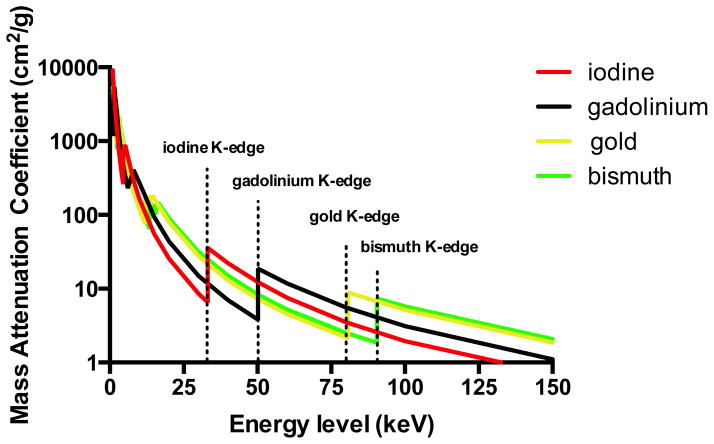
\includegraphics[scale=0.8]{./figuras/bode_k.jpg}
\caption{Ilustración bordes K (\textit{k-edge}) para distintos materiales. La figura se recuperó de la web \url{https://europepmc.org/article/PMC/4467470}.}
\label{fig:p6}
\end{figure}
Este concepto se relaciona con la probabilidad de que ocurra el efecto fotoeléctrico, el rayos X que incide a algún material debe tener al menos igual o mayor que la energía de enlace del electrón de la capa interna, observemos en la figura \ref{fig:p6} que la absorción de fotones aumenta mucho a medida que la energía de los fotones de rayos X que inciden aumenta desde abajo hacia arriba de la energía de enlace de los electrones de la capa K, lo cual es referido como el borde K. Como se muestra en la figura \ref{fig:p6}, la energía de enlace de los electrones en la capa K, o sea el borde K, según el átomo es distinta. Entonces, el efecto fotoeléctrico predomina en energía por encima del borde K del blanco y la ésta probabilidad aumenta según el número atómico crece: yodo (\ec{Z=53}), gadolinio (\ec{Z=64}), oro (\ec{Z=79}), bismuto (\ec{Z=83}); según la figura \ref{fig:p6}.



\item ¿Qué es el efecto talón?

Efecto tacón
Como los rayos X  producidos dentro del ánodo  viajan por igual en todas las direcciones,  dentro del ánodo deben atravesar una parte del objetivo y se atenúan a medida que salen del material del ánodo. La atenuación es mayor en la dirección del ánodo que en la dirección del cátodo (ver figura \ref{fig:p3}) y eso es provocado por la diferencia de longitud dentro del blanco: lo anterior es el efecto talón, entonces, tendremos una mayor intensidad de rayos X en el extremo del cátodo y menor intensidad en la del ánodo, por geometría,  la magnitud de este efecto depende del ángulo del ánodo o angulación, la distancia entre el detector de la fuente a la imagen y el tamaño del campo de radiación.

\item ¿Qué es la eficiencia cuántica de un detector?

La eficiencia cuántica del detector \ec{\eta_Q} es la fracción de los fotones que inciden a un detector con respecto a cuántos se han registrado, dada en la ec. \ref{e:p8}, con \ec{\mu_d} el coeficientes lineal de atenuación del detector y \ec{D} el espesor del detector, siempre se satisface que \ec{\eta_Q<1} ya que el detector no es ideal, aunque es posible aumentar \ec{\mu_d} y \ec{D} para tener un \ec{\eta_Q} cercano a \ec{1}, sin embargo, aplicar lo último nos llevará a tener un deterioro de la imagen ya que perderemos resolución espacial.

\eq{e:p8}{\eta_Q=1-e^{\mu_dD}}




\pagebreak

\item Con tus propias palabras, ¿Cuál es la relevancia del contraste? ¿Cómo se relaciona con todos los conceptos que se han discutido en la clase?


El contraste se refiere a la diferencia de intensidades en dos pixeles, en la imagen, por ejemplo: el contraste nos permite comparar la intensidad en los pixeles donde hay una lesión con la intensidad de los tejidos alrededor de la lesión.  En la radiografías el contraste se da  como resultado  por el contraste dado por el sujeto con el contraste dado por el dispositivo de detección y cómo se visualiza la imagen, en cuanto las imágenes digitales, se tendrá la ventaja de que el contraste se puede ajustar automáticamente después de obtener la imagen por el médico, sin embargo, esto no garantizará que siempre el contraste nos muestre las diferencias importantes para realizar las observaciones necesarias ya que el manejo de los dispositivos de detección o  de radiación dispersa o absorbida o ajuste de  los detectores no siempre será la adecuada dándonos imágenes con posibles artefactos o pobre resolución espacial.











\item ¿Cuáles son los dos tipos de filtros utilizados en radiodiagnóstico? ¿Cómo afectan en un espectro de energías?
\end{enumerate}


El filtrado consiste eliminar los rayos de baja energía que no es de aportación a la imagen médica, su objetivo es aumentar la energía promedio (o calidad) del haz de rayos X.  Se usan dos tipos de filtro en rayos X:
\begin{itemize}
  \item \textbf{Filtro inherente}: Este filtro viene incluido en el sistema de generación del haz de rayos X, consiste en una ventana de berilio y en el espectro elimina rayos X débiles, en la curva de la figura \ref{fig:p10} se observa este comportamiento.
  \item \textbf{Filtro añadido}: Es un filtro adicional y externo al sistema de generación de haces de rayos X y consisten de láminas que eliminan los rayos X que tienen suficiente energía para pasar a través de la filtración inherente pero que aún no son lo suficientemente energéticos para contribuir a la formación de imágenes, en la curva roja se observa el comportamiento de este filtro, la cual está aplicada también el comportamiento del filtro inherente.
\end{itemize}
%

\begin{figure}[!ht]
  \center
  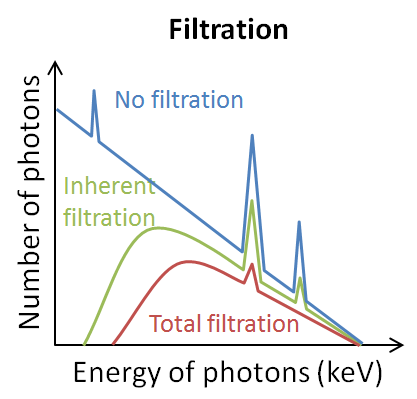
\includegraphics[scale=0.8]{./figuras/filtro.png}
  \caption{Ilustración del uso de filtros. La figura se recuperó de la web \url{https://sites.google.com/site/frcrphysicsnotes/production-of-x-rays}.}
  \label{fig:p10}
  \end{figure}

%\begin{multicols}{2}
%\small{\bibliographystyle{apalike}
%\bibliography{bib}}
%\end{multicols}



%\ftikz{1.5}{figuras/fig.tikz}{}{fig:x}

\end{document}



